%%%%%%%%%%%%%%%%%%%%%%%%%%%%%%%%%%%%%%%%%%%%%%%%%%%%%%%%
\fondo{celeste}
\section{¿Qué es una imagen?}
\fondo{blanco}
%%%%%%%%%%%%%%%%%%%%%%%%%%%%%%%%%%%%%%%%%%%%%%%%%%%%%%%%

%%%%%%%%%%%%%%%%%%%%%%%%%%%%%%%%%%%%%%%%%%%%%%%%%%%%%%%%
\begin{frame}
    \frametitle{¿Qué es una imagen?}
    \begin{block}{}
        Una imagen digital se representa como una matriz de valores, donde cada elemento (píxel) de la matriz almacena la intensidad de luz en un punto específico de la imagen.
    \end{block}

\begin{center}
    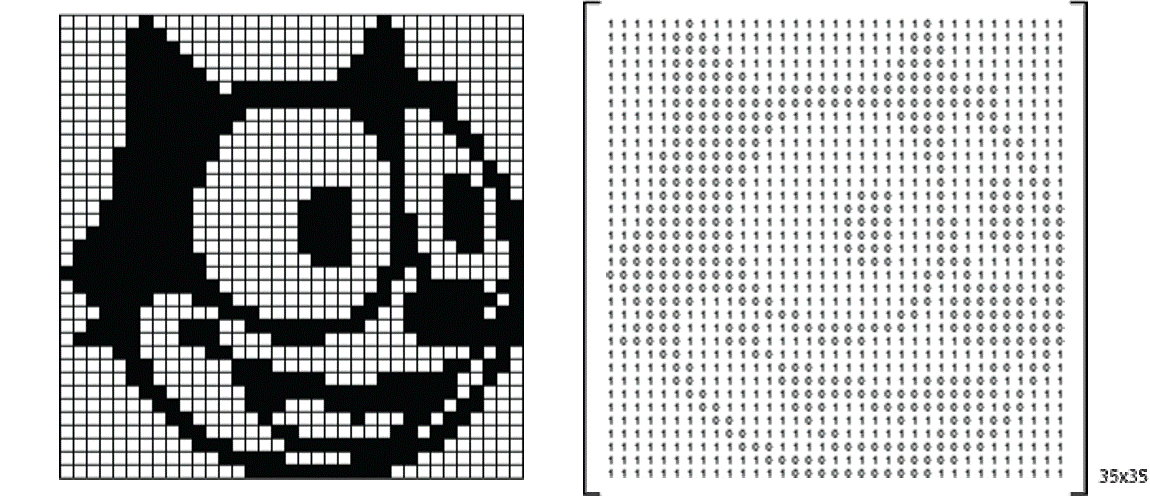
\includegraphics[width=9.5cm]{Figuras/Img01}
\end{center}


\end{frame}
%%%%%%%%%%%%%%%%%%%%%%%%%%%%%%%%%%%%%%%%%%%%%%%%%%%%%%%%

%%%%%%%%%%%%%%%%%%%%%%%%%%%%%%%%%%%%%%%%%%%%%%%%%%%%%%%%
\begin{frame}{El formato RGB}
    \begin{columns}
    \column{.5\textwidth}
    \begin{itemize}
        \item 
        Modelo de color basado en la síntesis aditiva
        \item 
        Es posible representar un color mediante la mezcla por adición de los tres colores de luz primarios: \textcolor{red}{rojo}, \textcolor{green}{verde} o \textcolor{azul}{azul}.
        \item 
        Tiene rangos de 0 a 255 (enteros) o de 0 a 1 (reales).
    \end{itemize}
    \column{.5\textwidth}
        \postitimg[6cm]{Figuras/Img02} % Inserta la figura correspondiente
    \end{columns}
\end{frame}
%%%%%%%%%%%%%%%%%%%%%%%%%%%%%%%%%%%%%%%%%%%%%%%%%%%%%%%%

%%%%%%%%%%%%%%%%%%%%%%%%%%%%%%%%%%%%%%%%%%%%%%%%%%%%%%%%
\begin{frame}{Ejemplo}
    \[
        R = \begin{pmatrix}
            0.0& 0.3& 0.9\\
            1.0& 0.0& 1.0
        \end{pmatrix};\quad
        G = \begin{pmatrix}
            0.0& 0.3& 0.3\\
            0.0& 1.0& 1.0
        \end{pmatrix};\quad
        B = \begin{pmatrix}
            0.0& 0.3& 0.9\\
            0.0& 0.0& 1.0
        \end{pmatrix}.
    \]
    \pause  
    \begin{center}
    \postitimg[5cm]{Figuras/Img03} % Inserta la figura correspondiente
    \end{center}
\end{frame}
%%%%%%%%%%%%%%%%%%%%%%%%%%%%%%%%%%%%%%%%%%%%%%%%%%%%%%%%

%%%%%%%%%%%%%%%%%%%%%%%%%%%%%%%%%%%%%%%%%%%%%%%%%%%%%%%%
\begin{frame}[fragile]
    \frametitle{Mejorar imágenes}

    \begin{center}
    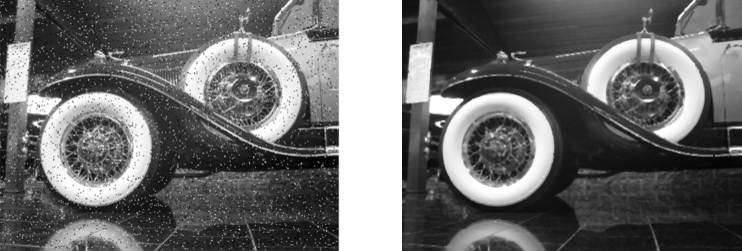
\includegraphics[width=9cm]{Figuras/Img04.png}

    \footnotesize
    \begin{tikzpicture}
    % Left matrix
    \matrix[matrix of nodes, nodes={draw, minimum size=0.8cm, anchor=center}, column sep=-\pgflinewidth, row sep=-\pgflinewidth] (A) {
        82 & 81 & 82\\
        81 & \color{purple}200 & 83 \\
        80 & 83 & 84 \\
    };
    
    % Green arrows pointing to the red value
    \foreach \i in {1,2,3} {
        \draw[->, thick, celeste, shorten >=-6pt, shorten <=-3pt] (A-\i-1) -- (A-2-2);
        \draw[->, thick, celeste, shorten >=-6pt, shorten <=-3pt] (A-\i-3) -- (A-2-2);
    }
    \foreach \i in {1,3} {
        \draw[->, thick, celeste, shorten >=-6pt, shorten <=-3pt] (A-\i-2) -- (A-2-2);
    }

    % Ordered list
    \node[draw, minimum height=0.8cm, right=4cm of A, anchor=center] (list) {
        \phantom{2}80 \quad 81 \quad 81 \quad 82 \quad \textcolor{celeste}{82} \quad 83 \quad 83 \quad 84 \quad 200
    };

    % Label 'Ordered List'
    \node[above=0.2cm of list] {Lista ordenada};

    % Arrow pointing to ordered list
    \draw[->, thick] (A) -- (list);

    % Arrow and label 'selected value'
    \draw[->, thick] (list.south) -- ++(0, -0.5) node[below] {valor seleccionado};

    % Right matrix
    \matrix[matrix of nodes, nodes={draw, minimum size=0.8cm, anchor=center}, right=8cm of A, column sep=-\pgflinewidth, row sep=-\pgflinewidth] (B) {
        \node {82}; & \node {81}; & \node {82}; \\
        \node {81}; & \node {\textcolor{celeste}{82}}; & \node {83}; \\
        \node {80}; & \node {83}; & \node {84}; \\
    };

    % Arrow pointing to right matrix
    \draw[->, thick] (list.east) -- (B);
\end{tikzpicture}

    \end{center}
\end{frame}

%%%%%%%%%%%%%%%%%%%%%%%%%%%%%%%%%%%%%%%%%%%%%%%%%%%%%%%%
\begin{frame}
    \frametitle{Un par más de conceptos}

    \begin{columns}
    \column{.5\textwidth}
    \begin{block}{Bounding Box}
        \begin{itemize}
            \item Delimita un objeto dentro de una imagen utilizando un rectángulo.
            \item Proporciona coordenadas $(x, y)$ y dimensiones $($ancho, alto$)$ del rectángulo.
        \end{itemize}
    \end{block}

    \column{.5\textwidth}

    \begin{tikzpicture}
    % Draw axes
    \draw[->, celeste] (-0.5,5) -- (4.5,5) node[right] {$x$};
    \draw[->, celeste] (0,5.5) -- (0,-0.5) node[right] {$y$};
    % (0,0) point and arrow
    \node[celeste, above left] at (0,5) {$(0,0)$};
    
    % Frame box
    \draw[thick, azul] (0,0) rectangle (4,5);
    
    % Bounding box
    \draw[thick, dashed] (1.5,3) rectangle (3,1);
    % (x,y) point and arrow
    \draw[dashed, celeste] (0,3) -- (1.5,3) -- (1.5,5);
    \fill[celeste] (1.5,3) circle (2pt);
    \node[celeste, above left] at (1.5,3) {$(x,y)$};
    
    \node at (2.25,2) {\scalebox{3.4}[5.2]{\color{azul}\faUmbrella}};
    \node[above right] at (1.5,3) {\footnotesize Bounding box};
    
    \draw[<->] (1.5,0.8) -- (3,0.8);
    \node[below] at (2.25,0.8) {\footnotesize ancho};
    
    \draw[<->] (3.2,1) -- (3.2,3);
    \node[right] at (3.2,2) {\rotatebox{90}{\footnotesize alto}};
    
    \end{tikzpicture}

    \end{columns}
    
\end{frame}
%%%%%%%%%%%%%%%%%%%%%%%%%%%%%%%%%%%%%%%%%%%%%%%%%%%%%%%%
%%%%%%%%%%%%%%%%%%%%%%%%%%%%%%%%%%%%%%%%%%%%%%%%%%%%%%%%
\begin{frame}
    \frametitle{Un par más de conceptos}

    \begin{columns}
    \column{.5\textwidth}
    \begin{block}{Segmentación Semántica}
        \begin{itemize}
            \item Asigna una etiqueta a cada píxel de la imagen, clasificándolos según el tipo de objeto al que pertenecen.
            \item Proporciona una delimitación precisa de los contornos de los objetos.
        \end{itemize}
    \end{block}
    \column{.5\textwidth}
    \begin{center}
        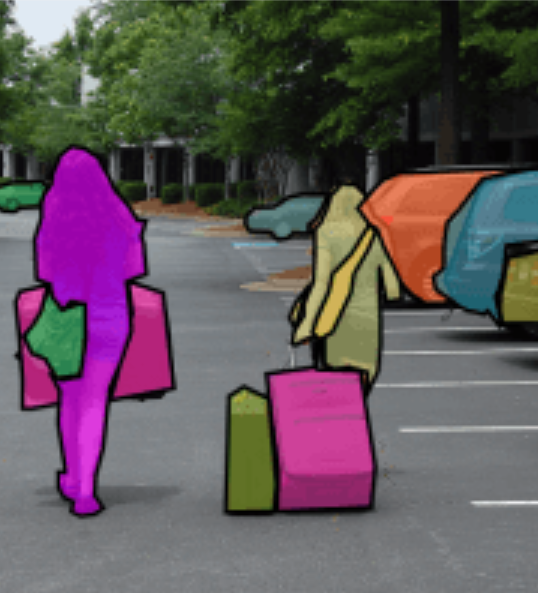
\includegraphics[width=5.5cm]{Figuras/Img05.png}
    \end{center}
    \end{columns}

\end{frame}
%%%%%%%%%%%%%%%%%%%%%%%%%%%%%%%%%%%%%%%%%%%%%%%%%%%%%%%%

%%%%%%%%%%%%%%%%%%%%%%%%%%%%%%%%%%%%%%%%%%%%%%%%%%%%%%%%
\begin{frame}
    \frametitle{¿Cómo aprende una máquina a interpretar una imagen?}

    \begin{block}{}
        \centering
        Una imagen no es más que una tabla de números. \\[0.4cm]
        ¿Cómo puede una computadora aprender, a partir de esos números, \\
        que está viendo una abeja, una mariposa o una flor?
    \end{block}

    \pause
    \vspace{0.4cm}
    \centering
    La respuesta: \textbf{redes neuronales convolucionales}.

\end{frame}
%%%%%%%%%%%%%%%%%%%%%%%%%%%%%%%%%%%%%%%%%%%%%%%%%%%%%%%%
